\newpage
\section{MC and data comparison}

\begin{figure}[ht]
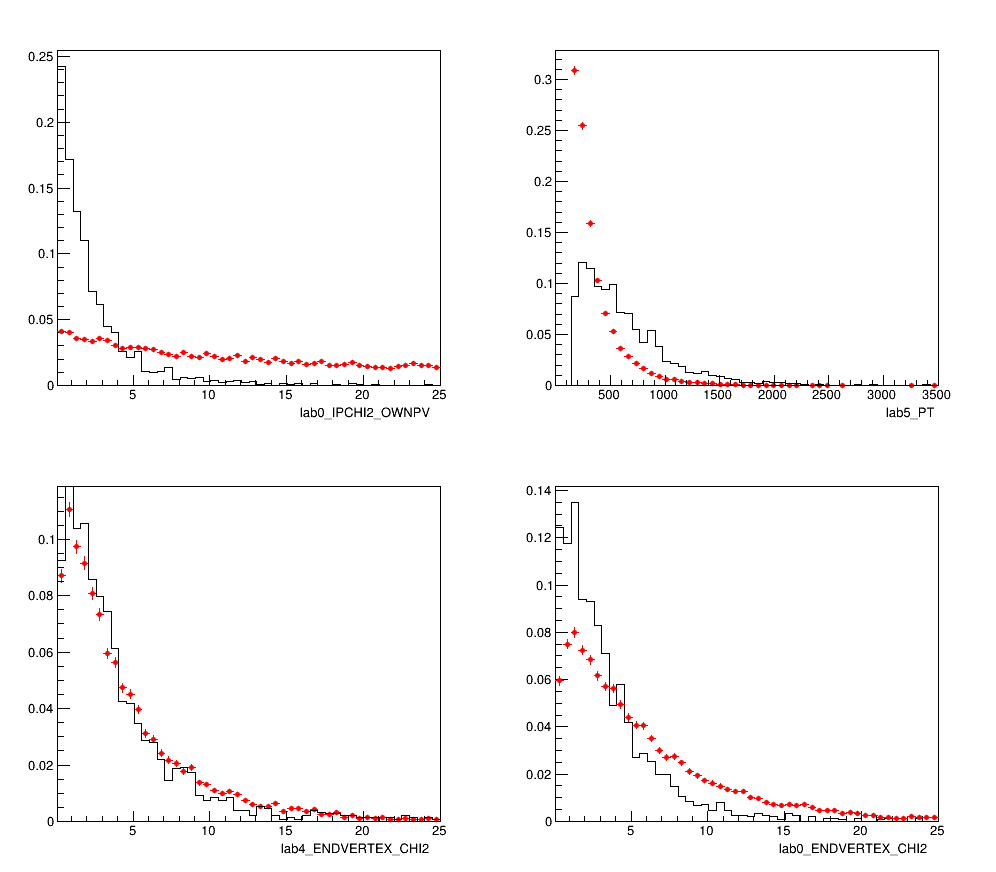
\includegraphics[width=11.5cm]{figs/MC_Data_Comp/DD0_0.png}
\centering
\caption{The comparison of simulated data (black lines) and Run 2 data (red dots) for selected variable, downstream tracks, data after preselection.}
\label{fig:MC_Data_Comp_DD0_0}
\end{figure}


\begin{figure}[hb]
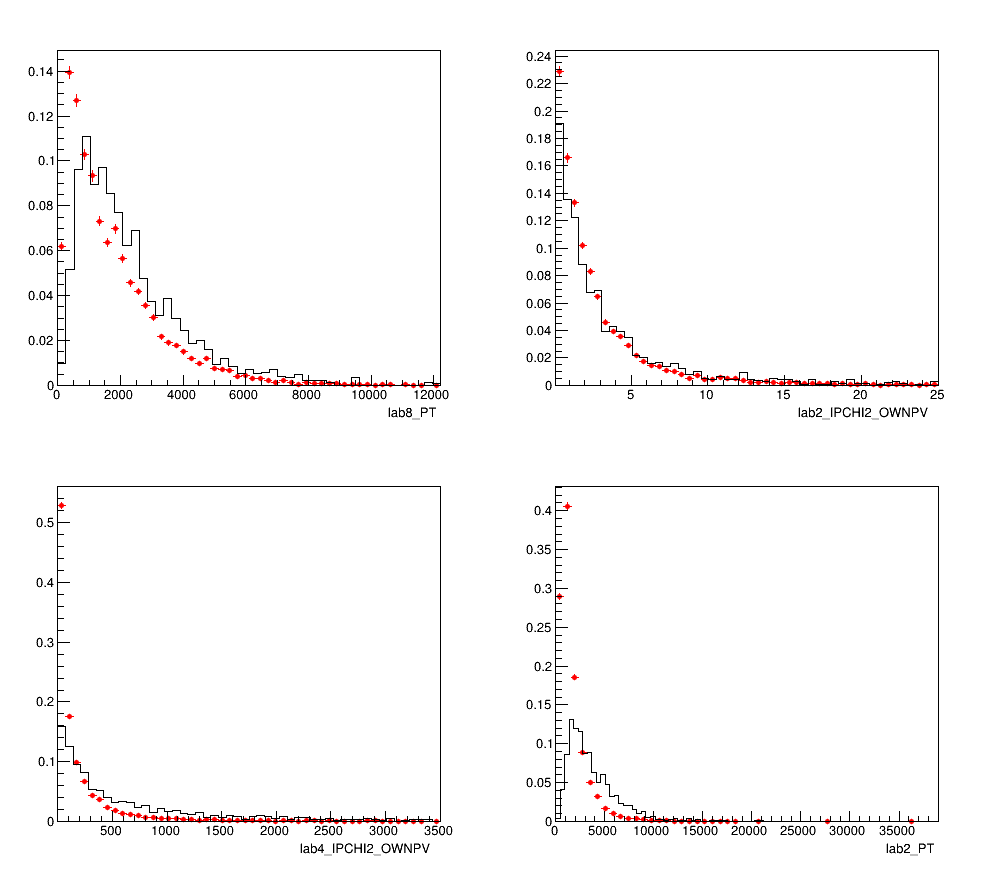
\includegraphics[width=11.5cm]{figs/MC_Data_Comp/DD0_1.png}
\centering
\caption{The comparison of simulated data (black lines) and Run 2 data (red dots) for selected variable, downstream tracks, data after preselection.}
\label{fig:MC_Data_Comp_DD0_1}
\end{figure}


\begin{figure}[ht]
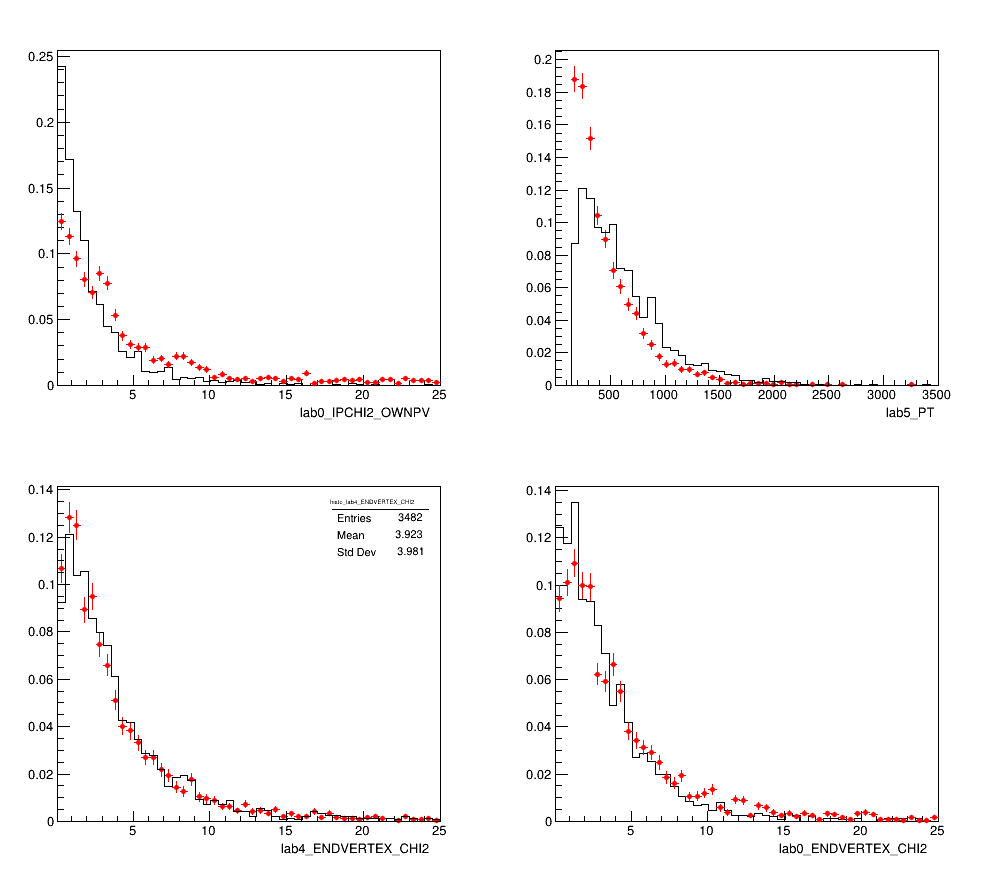
\includegraphics[width=11.5cm]{figs/MC_Data_Comp/DD1_0.png}
\centering
\caption{The comparison of simulated data (black lines) and Run 2 data (red dots) for selected variable, downstream tracks, data after preselection and BDT cut: BDT$>$0.1}
\label{fig:MC_Data_Comp_DD1_0}
\end{figure}


\begin{figure}[hb]
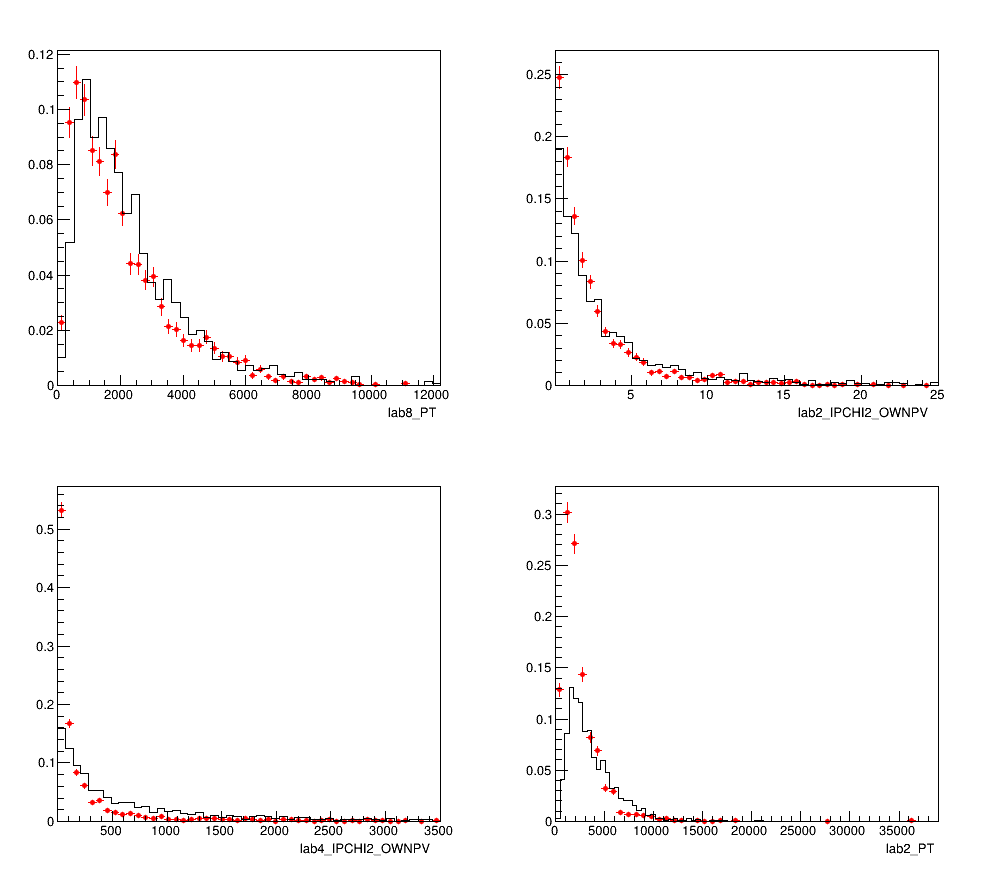
\includegraphics[width=11.8cm]{figs/MC_Data_Comp/DD1_1.png}
\centering
\caption{The comparison of simulated data (black lines) and Run 2 data (red dots) for selected variable, downstream tracks, data after preselection and BDT cut: BDT$>$0.1}
\label{fig:MC_Data_Comp_DD1_1}
\end{figure}


\begin{figure}[ht]
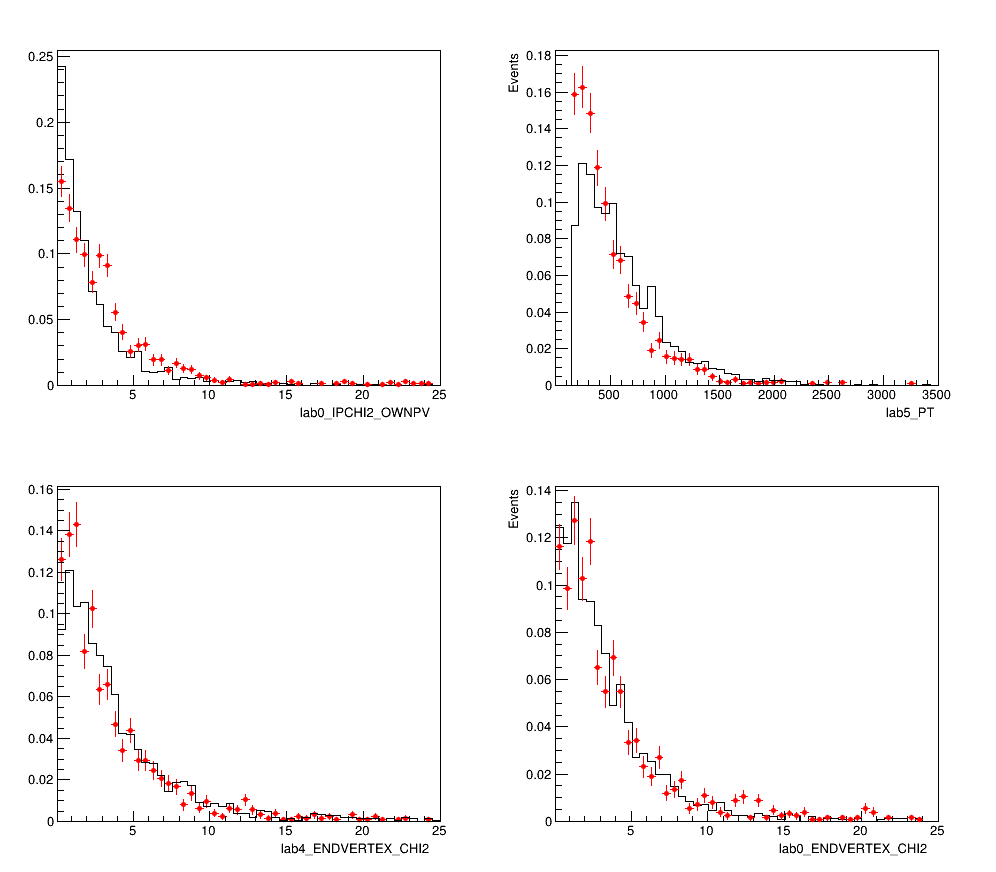
\includegraphics[width=11.5cm]{figs/MC_Data_Comp/DD8_0.png}
\centering
\caption{The comparison of simulated data (black lines) and Run 2 data (red dots) for selected variable, downstream tracks, data after preselection and BDT cut: BDT$>$0.8}
\label{fig:MC_Data_Comp_DD2_0}
\end{figure}


\begin{figure}[hb]
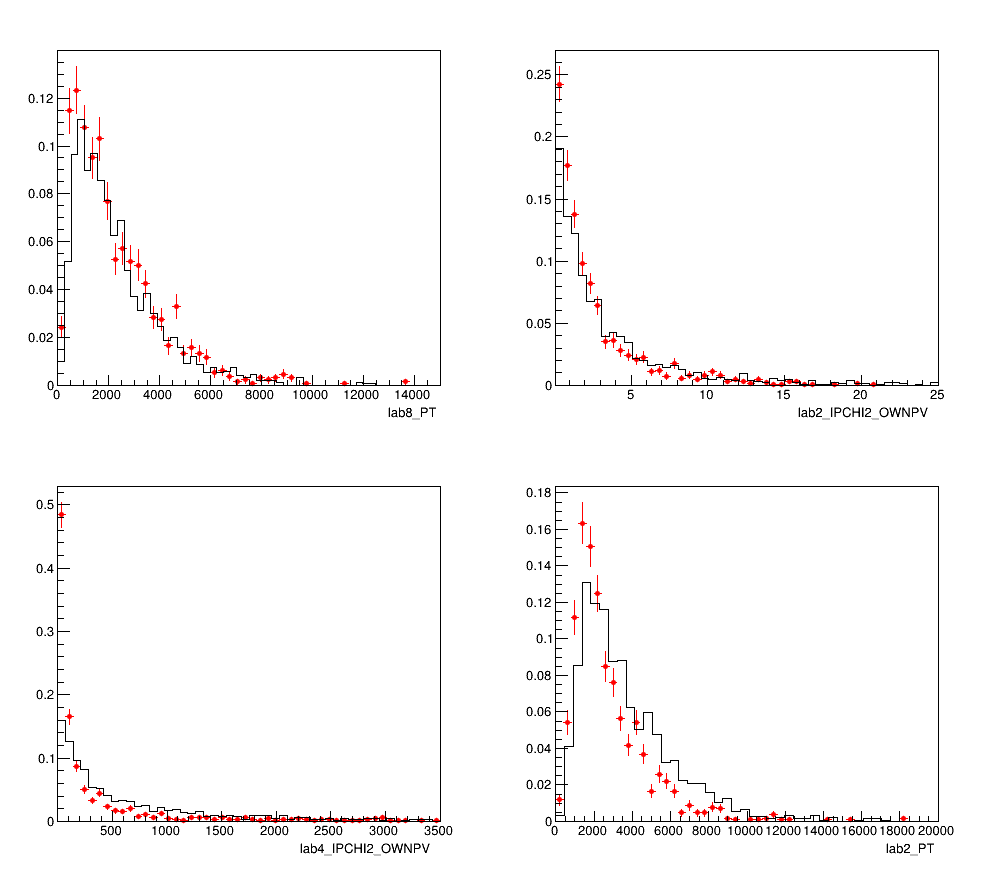
\includegraphics[width=11.5cm]{figs/MC_Data_Comp/DD8_1.png}
\centering
\caption{The comparison of simulated data (black lines) and Run 2 data (red dots) for selected variable, downstream tracks, data after preselection and BDT cut: BDT$>$0.8}
\label{fig:MC_Data_Comp_DD2_1}
\end{figure}


\begin{figure}[ht]
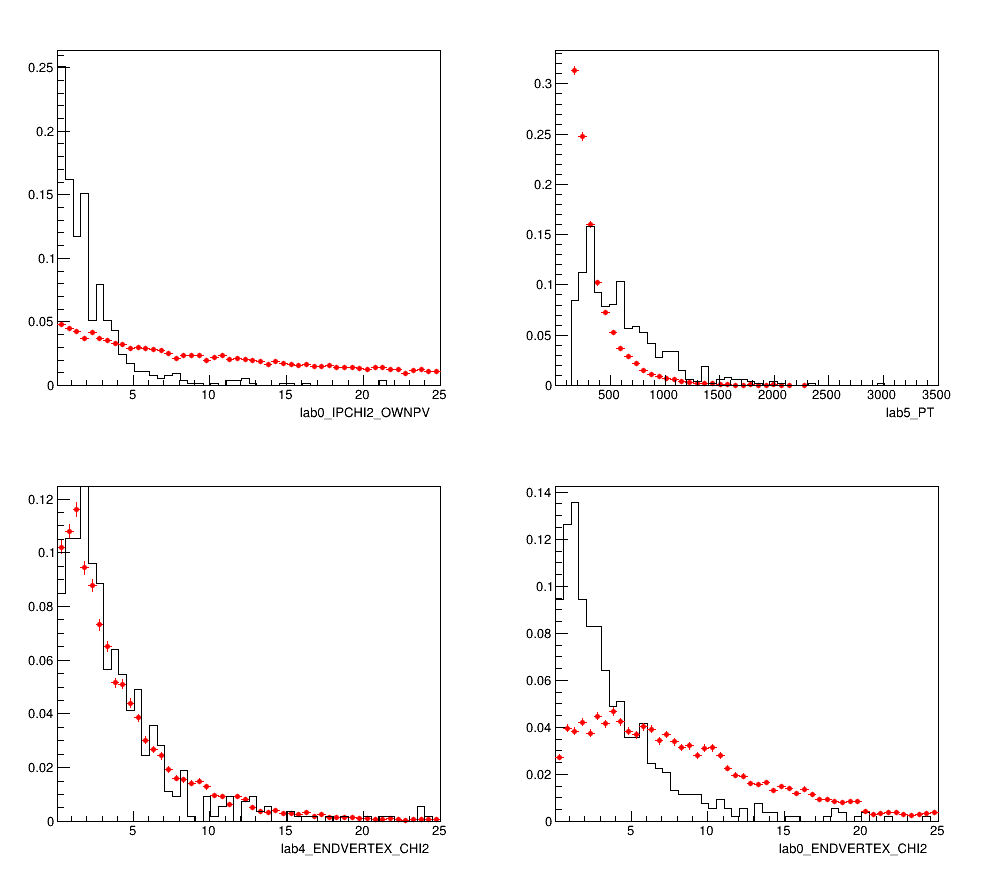
\includegraphics[width=11.5cm]{figs/MC_Data_Comp/LL0_0.png}
\centering
\caption{The comparison of simulated data (black lines) and Run 2 data (red dots) for selected variable, long tracks, data after preselection.}
\label{fig:MC_Data_Comp_LL0_0}
\end{figure}


\begin{figure}[hb]
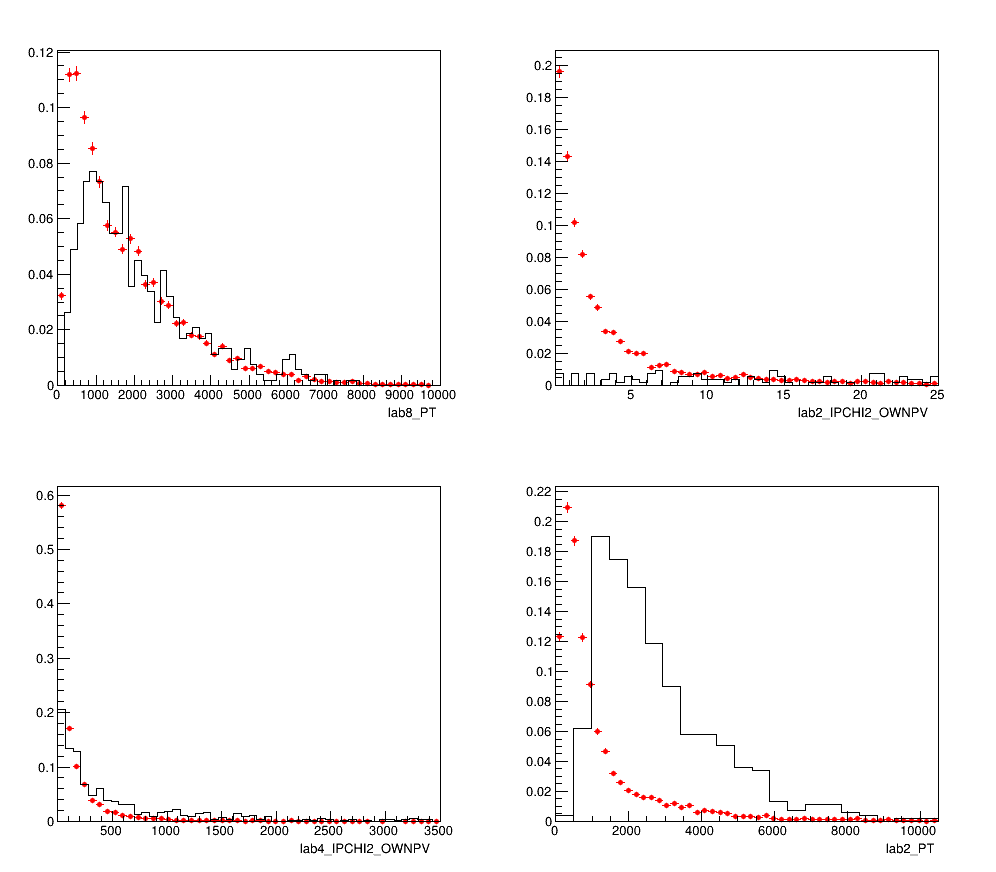
\includegraphics[width=11.5cm]{figs/MC_Data_Comp/LL0_1.png}
\centering
\caption{The comparison of simulated data (black lines) and Run 2 data (red dots) for selected variable, long tracks, data after preselection.}
\label{fig:MC_Data_Comp_LL0_1}
\end{figure}


\begin{figure}[ht]
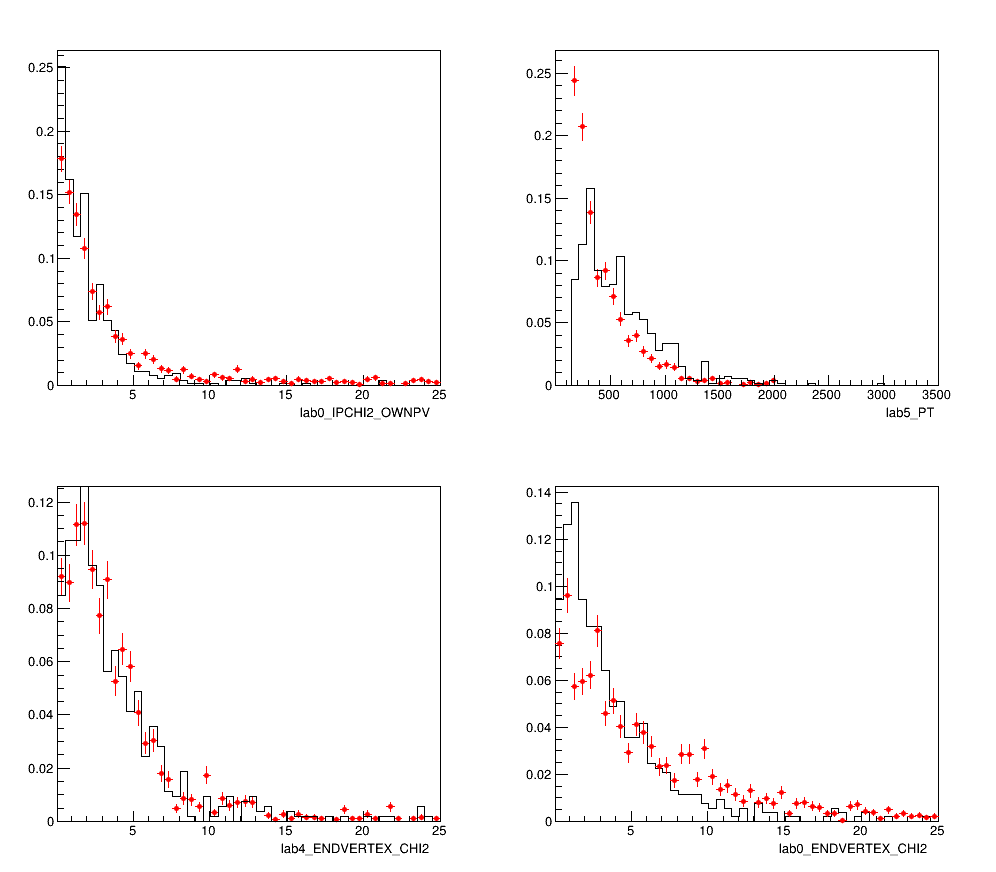
\includegraphics[width=11.5cm]{figs/MC_Data_Comp/LL1_0.png}
\centering
\caption{The comparison of simulated data (black lines) and Run 2 data (red dots) for selected variable, long tracks, data after preselection and BDT cut: BDT$>$0.1}
\label{fig:MC_Data_Comp_LL1_0}
\end{figure}


\begin{figure}[hb]
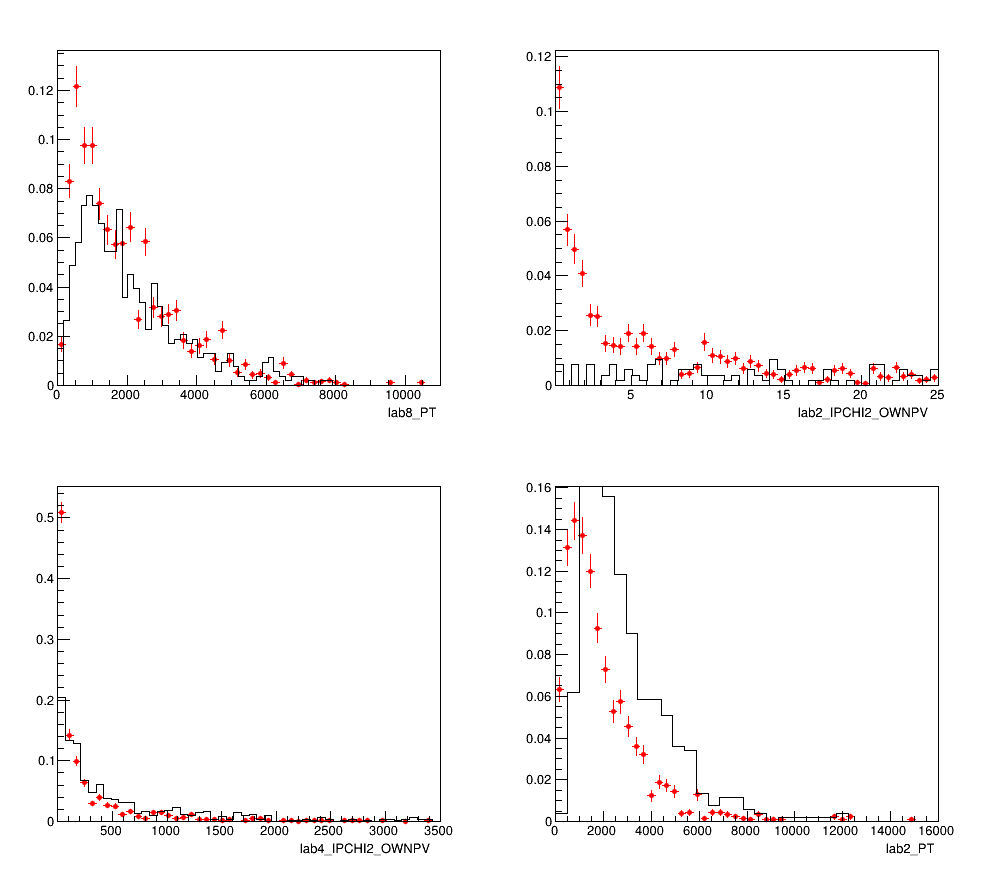
\includegraphics[width=11.5cm]{figs/MC_Data_Comp/LL1_1.png}
\centering
\caption{The comparison of simulated data (black lines) and Run 2 data (red dots) for selected variable, long tracks, data after preselection and BDT cut: BDT$>$0.1}
\label{fig:MC_Data_Comp_LL1_1}
\end{figure}


\begin{figure}[ht]
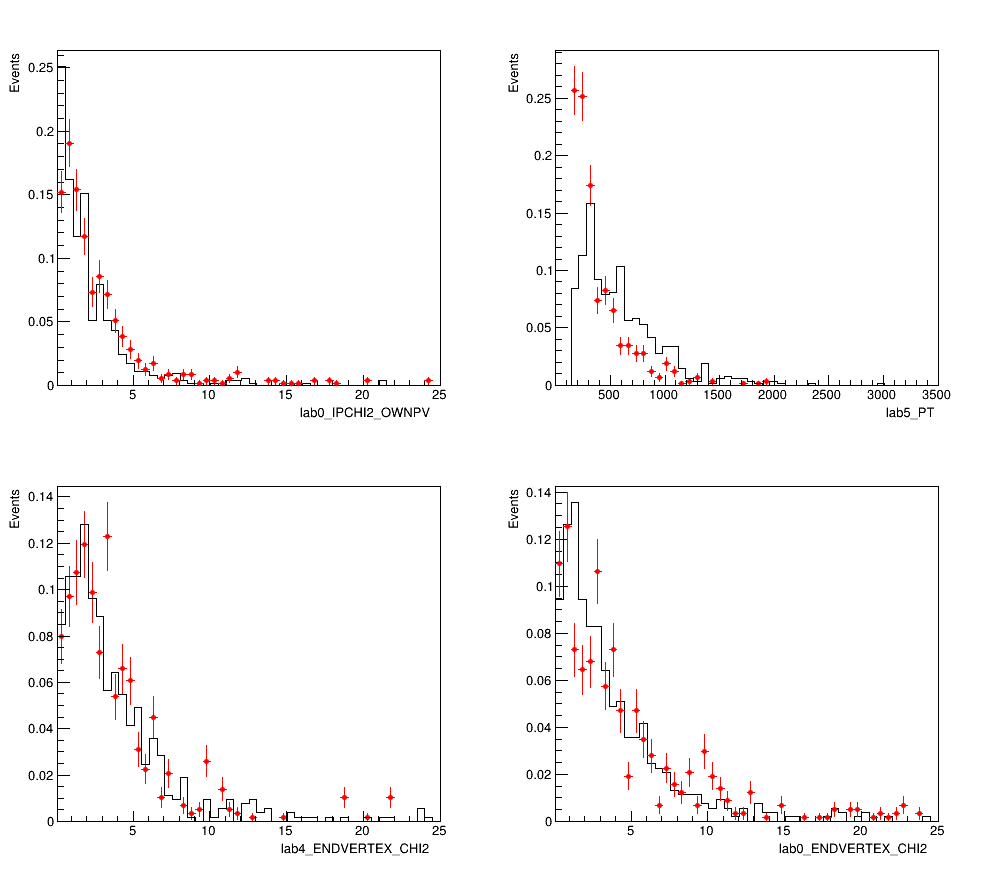
\includegraphics[width=11.5cm]{figs/MC_Data_Comp/LL8_0.png}
\centering
\caption{The comparison of simulated data (black lines) and Run 2 data (red dots) for selected variable, long tracks, data after preselection and BDT cut: BDT$>$0.8}
\label{fig:MC_Data_Comp_LL2_0}
\end{figure}


\begin{figure}[hb]
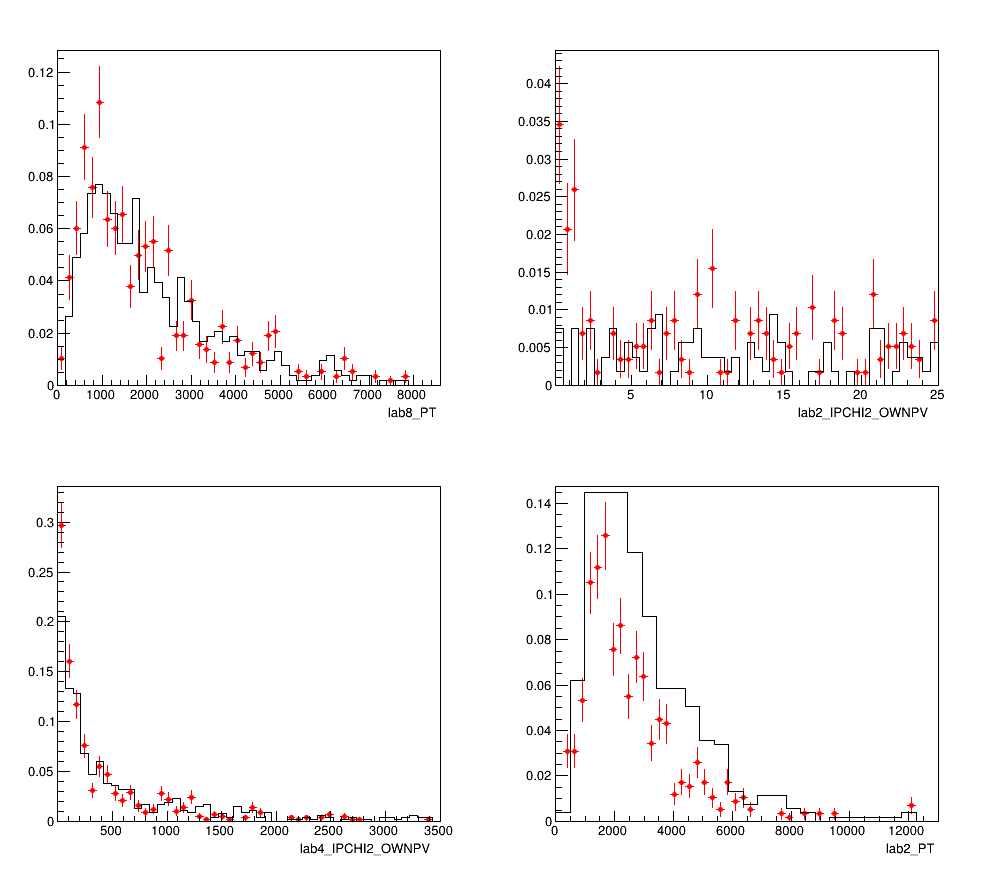
\includegraphics[width=11.5cm]{figs/MC_Data_Comp/LL8_1.png}
\centering
\caption{The comparison of simulated data (black lines) and Run 2 data (red dots) for selected variable, long tracks, data after preselection and BDT cut: BDT$>$0.8}
\label{fig:MC_Data_Comp_LL2_1}
\end{figure}

\newpage
